% !TeX spellcheck = en_US
% !TEX root = Ausarbeitung.tex

\section{Initial data exploration}
\subsection{Attribute features}
\subsubsection{Quote\_Id}
\paragraph{Attribute type: nominal}
The "Quote\_Id" is a customer number. It is neither orderable nor is the number a quantitative value.
\paragraph{Statistics: } As the attribute is nominal you can not perform any mathematical calculations. The Id ranges between 638 to 434297.

\subsubsection{Quote\_Date}
\paragraph{Attribute type: interval}
"Quote\_Date" seems to be at date. These have a specified point of zero. Therefore the type of the attribute is scale.
\paragraph{Statistics: } 
\textbf{Missing Values}: None

\textbf{Range}: $02/01/2013 - 18/05/2015$


\subsubsection{Quote\_Flag}
\paragraph{Attribute type: nominal (dichotomous)}
The description of the attributes declares "Quote\_Flag" as information about whether an insurance was purchased. This can be only answered with yes or no.
\paragraph{Statistics: }
\textbf{Missing Values}: None

\begin{table}[H]
	\renewcommand{\arraystretch}{1.25}
		\begin{tabular}{l|l|l}
			\textbf{Value} & \textbf{Absolute Frequency} & \textbf{Relative Frequency}\\\hline
			0 & $1605$ & $0.8025$\\ \hline
			1 & $395$ & $0.1975$\\
		\end{tabular}
\end{table}


\subsection{Field\_Info1}
\paragraph{Attribute type: nominal}
\paragraph{Statistics: }
\textbf{Missing Values}: None

\begin{table}[H]
	\renewcommand{\arraystretch}{1.25}
	\begin{tabular}{l|l|l}
		\textbf{Value} & \textbf{Absolute Frequency} & \textbf{Relative Frequency}\\\hline
			J&$390$ & $0.365$\\\hline
			F&$540$ & $0.27$\\\hline
			B&$730$ & $0.195$\\\hline
			E&$200$ & $0.1$\\\hline
			C&$39$ & $0.0505$\\\hline
			K&$101$ & $0.0195$\\
	\end{tabular}
\end{table}


\subsection{Field\_Info2}
\paragraph{Attribute type: ratio}
All values of "Field\_Info2" are numbers between $0$ and $2$ and have a precision of 4 decimals. This suggests that the values are on a zero-based scale.
\paragraph{Statistics: }
\begin{table}[H]
	\renewcommand{\arraystretch}{1.25}
	\begin{tabular}{l|l}
		\textbf{Statistic} & \textbf{Value}\\\hline
			Missing Values& None\\\hline
			Minimum& $0.8746$\\\hline
			Maximum& $1.0101$\\\hline
			Mean& $0.9391$\\\hline
			Std. Dev.& $0.0373$\\\hline
			90th Perc. & $1.00051$\\\hline
			10th Perc. & $0.8922$ \\
	\end{tabular}
\end{table}

\paragraph{Histrogramm}:

\subsection{Field\_Info3}
\paragraph{Attribute type: interval}
\paragraph{Statistics: }
\begin{table}[H]
	\renewcommand{\arraystretch}{1.25}
	\begin{tabular}{l|l}
		\textbf{Statistic} & \textbf{Value}\\\hline
		Missing Values& None\\\hline
	\end{tabular}
\end{table}

\subsection{Field\_Info4}
\paragraph{Attribute type: nominal (dichotomous)} In this Attribute only the values "Y" and "N" appear. Those values are often used as a short version on "Yes" and "No". This field therefore seems to be a yes-no answer.
\qquad
\begin{table}[H]
	\renewcommand{\arraystretch}{1.25}
	\begin{tabular}{l|l}
		\textbf{Statistic} & \textbf{Value}\\\hline
		Missing Values& None\\\hline
	\end{tabular}
\end{table}
\begin{table}[H]
	\renewcommand{\arraystretch}{1.25}
	\begin{tabular}{l|l|l}
		\textbf{Value} & \textbf{Absolute Frequency} & \textbf{Relative Frequency}\\\hline
		N	&$1860$&$0.93$\\\hline
		Y&	$140$&$0.07$
	\end{tabular}
\end{table}

\subsection{Coverage\_Info1}
\paragraph{Attribute type: interval/ordinal}\qquad

\begin{table}[H]
	\renewcommand{\arraystretch}{1.25}
	\begin{tabular}{l|l}
		\textbf{Statistic} & \textbf{Value}\\\hline
		Missing Values& None\\\hline
	\end{tabular}
\end{table}

\subsection{Coverage\_Info2}
\paragraph{Attribute type: interval/ordinal}
\paragraph{Statistics: }
\begin{table}[H]
	\renewcommand{\arraystretch}{1.25}
	\begin{tabular}{l|l}
		\textbf{Statistic} & \textbf{Value}\\\hline
		Missing Values& None\\\hline
	\end{tabular}
\end{table}

\subsection{Coverage\_Info3}
\paragraph{Attribute type: ordinal}
Alphabet, is a order
\qquad

\begin{table}[H]
	\renewcommand{\arraystretch}{1.25}
	\begin{tabular}{l|l}
		\textbf{Statistic} & \textbf{Value}\\\hline
		Missing Values& None\\\hline
	\end{tabular}
\end{table}
\begin{table}[H]
	\renewcommand{\arraystretch}{1.25}
	\begin{tabular}{l|l|l}
		\textbf{Value} & \textbf{Absolute Frequency} & \textbf{Relative Frequency}\\\hline
E&$673$&$0.3365$\\\hline
D&$388$&$0.194$\\\hline
G&$245$&$0.1225$\\\hline
K&$229$&$0.1145$\\\hline
F&$221$&$0.1105$\\\hline
A&$116$&$0.058$\\\hline
J&$110$&$0.055$\\\hline
I&$7$&$0.0035$\\\hline
B&$4$&$0.002$\\\hline
C&$3$&$0.0015$\\\hline
H&$2$&$0.001$\\\hline
L&$2$&$0.001$
	\end{tabular}
\end{table}

\subsection{Sales\_Info1}
\paragraph{Attribute type: nominal (dichotomous)}
\qquad
\begin{table}[H]
	\renewcommand{\arraystretch}{1.25}
	\begin{tabular}{l|l}
		\textbf{Statistic} & \textbf{Value}\\\hline
		Missing Values& None\\\hline
	\end{tabular}
\end{table}
\begin{table}[H]
	\renewcommand{\arraystretch}{1.25}
	\begin{tabular}{l|l|l}
		\textbf{Value} & \textbf{Absolute Frequency} & \textbf{Relative Frequency}\\\hline
		1&$1490$&$0.745$\\\hline
		0&$510$&$0.255$
	\end{tabular}
\end{table}

\subsection{Sales\_Info2}
\paragraph{Attribute type: ordinal} prop missing 1
\qquad
\begin{table}[H]
	\renewcommand{\arraystretch}{1.25}
	\begin{tabular}{l|l}
		\textbf{Statistic} & \textbf{Value}\\\hline
		Missing Values& None\\\hline
	\end{tabular}
\end{table}
\begin{table}[H]
	\renewcommand{\arraystretch}{1.25}
	\begin{tabular}{l|l|l}
		\textbf{Value} & \textbf{Absolute Frequency} & \textbf{Relative Frequency}\\\hline
		5&$1093$&$0.5465$\\\hline
		3&$519$&$0.2595$\\\hline
		4&$295$&$0.1475$\\\hline
		2&$93$&$0.0465$
	\end{tabular}
\end{table}

\subsection{Sales\_Info3}
\paragraph{Attribute type: ordinal} with missing values 0 - 25

\qquad
\begin{table}[H]
	\renewcommand{\arraystretch}{1.25}
	\begin{tabular}{l|l}
		\textbf{Statistic} & \textbf{Value}\\\hline
		Missing Values& None\\\hline
	\end{tabular}
\end{table}

\subsection{Sales\_Info4}
\paragraph{Attribute type: nominal} Is only letters sems no order
\paragraph{Statistics: }
\begin{table}[H]
	\renewcommand{\arraystretch}{1.25}
	\begin{tabular}{l|l}
		\textbf{Statistic} & \textbf{Value}\\\hline
		Missing Values& None\\\hline
	\end{tabular}
\end{table}
\begin{table}[H]
	\renewcommand{\arraystretch}{1.25}
	\begin{tabular}{l|l|l}
		\textbf{Value} & \textbf{Absolute Frequency} & \textbf{Relative Frequency}\\\hline
		K&$410$&$0.205$\\\hline
		P&$376$&$0.188$\\\hline
		T&$332$&$0.166$\\\hline
		Q&$312$&$0.156$\\\hline
		V&$298$&$0.149$\\\hline
		R&$156$&$0.078$\\\hline
		M&$116$&$0.058$
	\end{tabular}
\end{table}

\subsection{Sales\_Info5}
\paragraph{Attribute type: ration} prop something with money
\paragraph{Statistics: }
\begin{table}[H]
	\renewcommand{\arraystretch}{1.25}
	\begin{tabular}{l|l}
		\textbf{Statistic} & \textbf{Value}\\\hline
		Missing Values& None\\\hline
	\end{tabular}
\end{table}

\subsection{Personal\_Info1}
\paragraph{Attribute type: nominal (dichotomous)}
\paragraph{Statistics: }
\begin{table}[H]
	\renewcommand{\arraystretch}{1.25}
	\begin{tabular}{l|l}
		\textbf{Statistic} & \textbf{Value}\\\hline
		Missing Values& None\\\hline
	\end{tabular}
\end{table}
\begin{table}[H]
	\renewcommand{\arraystretch}{1.25}
	\begin{tabular}{l|l|l}
		\textbf{Value} & \textbf{Absolute Frequency} & \textbf{Relative Frequency}\\\hline
		N&$1993$&$0.9965$\\\hline
		Y&$7$&$0.0035$
	\end{tabular}
\end{table}

\subsection{Personal\_Info2}
\paragraph{Attribute type: ordinal} missing values
\paragraph{Statistics: }
\begin{table}[H]
	\renewcommand{\arraystretch}{1.25}
	\begin{tabular}{l|l}
		\textbf{Statistic} & \textbf{Value}\\\hline
		Missing Values& None\\\hline
	\end{tabular}
\end{table}

\subsection{Personal\_Info3}
\paragraph{Attribute type: nominal} two letter combination
\paragraph{Statistics: }
\begin{table}[H]
	\renewcommand{\arraystretch}{1.25}
	\begin{tabular}{l|l}
		\textbf{Statistic} & \textbf{Value}\\\hline
		Missing Values& None\\\hline
	\end{tabular}
\end{table}
\begin{table}[H]
	\renewcommand{\arraystretch}{1.25}
	\begin{tabular}{l|l|l}
		\textbf{Value} & \textbf{Absolute Frequency} & \textbf{Relative Frequency}\\\hline
		ZA&$937$&$0.4685$\\\hline
		XR&$104$&$0.052$\\\hline
		XM&$81$&$0.0405$\\\hline
		XJ&$73$&$0.0365$\\\hline
		XD&$63$&$0.0315$\\\hline
		XX&$62$&$0.031$\\\hline
		XB&$59$&$0.0295$\\\hline
		YH&$58$&$0.029$\\\hline
		XH&$54$&$0.027$\\\hline
		ZT&$51$&$0.0255$\\\hline
		XO&$50$&$0.025$\\\hline
		ZF&$46$&$0.023$\\\hline
		ZR&$40$&$0.02$\\\hline
		ZN&$39$&$0.0195$\\\hline
		ZH&$37$&$0.0185$\\\hline
		XS&$35$&$0.0175$\\\hline
		YF&$29$&$0.0145$\\\hline
		XW&$23$&$0.0115$\\\hline
		ZG&$20$&$0.01$\\\hline
		XE&$20$&$0.01$\\\hline
		ZW&$18$&$0.009$\\\hline
		YE&$17$&$0.0085$\\\hline
		ZC&$16$&$0.008$\\\hline
		XC&$14$&$0.007$\\\hline
		XQ&$14$&$0.007$\\\hline
		XL&$7$&$0.0035$\\\hline
		ZE&$7$&$0.0035$\\\hline
		ZJ&$6$&$0.003$\\\hline
		XI&$5$&$0.0025$\\\hline
		ZD&$5$&$0.0025$\\\hline
		ZK&$4$&$0.002$\\\hline
		XZ&$4$&$0.002$\\\hline
		ZU&$2$&$0.001$
	\end{tabular}
\end{table}

\subsection{Personal\_Info4}
\paragraph{Attribute type: nominal (dichotomous)}
\paragraph{Statistics: }
\begin{table}[H]
	\renewcommand{\arraystretch}{1.25}
	\begin{tabular}{l|l}
		\textbf{Statistic} & \textbf{Value}\\\hline
		Missing Values& None\\\hline
	\end{tabular}
\end{table}
\begin{table}[H]
	\renewcommand{\arraystretch}{1.25}
	\begin{tabular}{l|l|l}
		\textbf{Value} & \textbf{Absolute Frequency} & \textbf{Relative Frequency}\\\hline
		0&$1999$&$0.9995$\\\hline
		1&$1$&$0.001$
	\end{tabular}
\end{table}

\subsection{Personal\_Info5}
\paragraph{Attribute type: ordinal} most infos missing
\paragraph{Statistics: }
\paragraph{Missing Values}: $966$

\subsection{Property\_Info1}
\paragraph{Attribute type: nominal (dichotomous)}
\paragraph{Statistics: }
\paragraph{Missing Values}: $1$
\begin{table}[H]
	\renewcommand{\arraystretch}{1.25}
	\begin{tabular}{l|l|l}
		\textbf{Value} & \textbf{Absolute Frequency} & \textbf{Relative Frequency}\\\hline
		N&$1738$&$0.869$\\\hline
		Y&$261$&$0.1305$
\end{tabular}
\end{table}

\subsection{Property\_Info2}
\paragraph{Attribute type: nominal}
\paragraph{Statistics: }
\begin{table}[H]
	\renewcommand{\arraystretch}{1.25}
	\begin{tabular}{l|l}
		\textbf{Statistic} & \textbf{Value}\\\hline
		Missing Values& None\\\hline
	\end{tabular}
\end{table}

\subsection{Property\_Info3}
\paragraph{Attribute type: nominal} random letters
\paragraph{Statistics: }
\begin{table}[H]
	\renewcommand{\arraystretch}{1.25}
	\begin{tabular}{l|l}
		\textbf{Statistic} & \textbf{Value}\\\hline
		Missing Values& None\\\hline
	\end{tabular}
\end{table}
\begin{table}[H]
	\renewcommand{\arraystretch}{1.25}
	\begin{tabular}{l|l|l}
		\textbf{Value} & \textbf{Absolute Frequency} & \textbf{Relative Frequency}\\\hline
		O&$573$&$0.2865$\\\hline
		R&$533$&$0.2665$\\\hline
		J&$285$&$0.1425$\\\hline
		D&$198$&$0.099$\\\hline
		S&$146$&$0.073$\\\hline
		N&$92$&$0.046$\\\hline
		I&$77$&$0.0385$\\\hline
		A&$31$&$0.0155$\\\hline
		Q&$30$&$0.015$\\\hline
		E&$10$&$0.005$\\\hline
		H&$9$&$0.0045$\\\hline
		K&$6$&$0.003$\\\hline
		F&$5$&$0.0025$\\\hline
		L&$3$&$0.0015$\\\hline
		G&$2$&$0.001$
	\end{tabular}
\end{table}

\subsection{Property\_Info4}
\paragraph{Attribute type: nominal (dichotomous)}
\paragraph{Statistics: }
\begin{table}[H]
	\renewcommand{\arraystretch}{1.25}
	\begin{tabular}{l|l}
		\textbf{Statistic} & \textbf{Value}\\\hline
		Missing Values& None\\\hline
	\end{tabular}
\end{table}
\begin{table}[H]
	\renewcommand{\arraystretch}{1.25}
	\begin{tabular}{l|l|l}
		\textbf{Value} & \textbf{Absolute Frequency} & \textbf{Relative Frequency}\\\hline
		1&$1364$&$0.682$\\\hline
		0&$636$&$0.318$
	\end{tabular}
\end{table}

\subsection{Property\_Info5}
\paragraph{Attribute type: interval}
\paragraph{Statistics: }
\begin{table}[H]
	\renewcommand{\arraystretch}{1.25}
	\begin{tabular}{l|l}
		\textbf{Statistic} & \textbf{Value}\\\hline
		Missing Values& None\\\hline
	\end{tabular}
\end{table}

\subsection{Geographic\_Info1}
\paragraph{Attribute type: ordinal}
\paragraph{Statistics: }
\begin{table}[H]
	\renewcommand{\arraystretch}{1.25}
	\begin{tabular}{l|l}
		\textbf{Statistic} & \textbf{Value}\\\hline
		Missing Values& None\\\hline
	\end{tabular}
\end{table}

\subsection{Geographic\_Info2}
\paragraph{Attribute type: interval}
\paragraph{Statistics: }
\begin{table}[H]
	\renewcommand{\arraystretch}{1.25}
	\begin{tabular}{l|l}
		\textbf{Statistic} & \textbf{Value}\\\hline
		Missing Values& None\\\hline
	\end{tabular}
\end{table}

\subsection{Geographic\_Info3}
\paragraph{Attribute type: nominal} probably is pullshit, could be info
\paragraph{Statistics: }
\begin{table}[H]
	\renewcommand{\arraystretch}{1.25}
	\begin{tabular}{l|l}
		\textbf{Statistic} & \textbf{Value}\\\hline
		Missing Values& None\\\hline
	\end{tabular}
\end{table}
\begin{table}[H]
	\renewcommand{\arraystretch}{1.25}
	\begin{tabular}{l|l|l}
		\textbf{Value} & \textbf{Absolute Frequency} & \textbf{Relative Frequency}\\\hline
		-1&$1942$&$0.971$\\hline
		25&$58$&$0.029$
	\end{tabular}
\end{table}

\subsection{Geographic\_Info4}
\paragraph{Attribute type: nominal (dichotomous)}
\paragraph{Statistics: }
\begin{table}[H]
	\renewcommand{\arraystretch}{1.25}
	\begin{tabular}{l|l}
		\textbf{Statistic} & \textbf{Value}\\\hline
		Missing Values& None\\\hline
	\end{tabular}
\end{table}
\begin{table}[H]
	\renewcommand{\arraystretch}{1.25}
	\begin{tabular}{l|l|l}
		\textbf{Value} & \textbf{Absolute Frequency} & \textbf{Relative Frequency}\\\hline
		N&$1961$&$0.9805$\\\hline
		Y&$39$&$0.0195$
	\end{tabular}
\end{table}

\subsection{Geographic\_Info5}
\paragraph{Attribute type: nominal} Could be states
\paragraph{Statistics: }
\begin{table}[H]
	\renewcommand{\arraystretch}{1.25}
	\begin{tabular}{l|l}
		\textbf{Statistic} & \textbf{Value}\\\hline
		Missing Values& None\\\hline
	\end{tabular}
\end{table}
\begin{table}[H]
	\renewcommand{\arraystretch}{1.25}
	\begin{tabular}{l|l|l}
		\textbf{Value} & \textbf{Absolute Frequency} & \textbf{Relative Frequency}\\\hline
		CA&$730$&$0.365$\\\hline
		NJ&$540$&$0.27$\\\hline
		TX&$491$&$0.2455$\\\hline
		IL&$239$&$0.1195$
	\end{tabular}
\end{table}

\section{Data Preprocessing}

\section{Summary}


\section{Projektinhalt}
\subsection{Aktivitäten}
\begin{table}[H]
    \renewcommand{\arraystretch}{1.05}
    \begin{center}
        \begin{tabular}{l|l}
            \hline
            \textbf{ID} & \textbf{Aktivität}\\\hline
            A & Projektmanager\\ \hline
        \end{tabular}
        \caption{Aktivitäten im Projekt}
    \end{center}
\end{table}

\begin{figure}[H]
    \begin{center}
        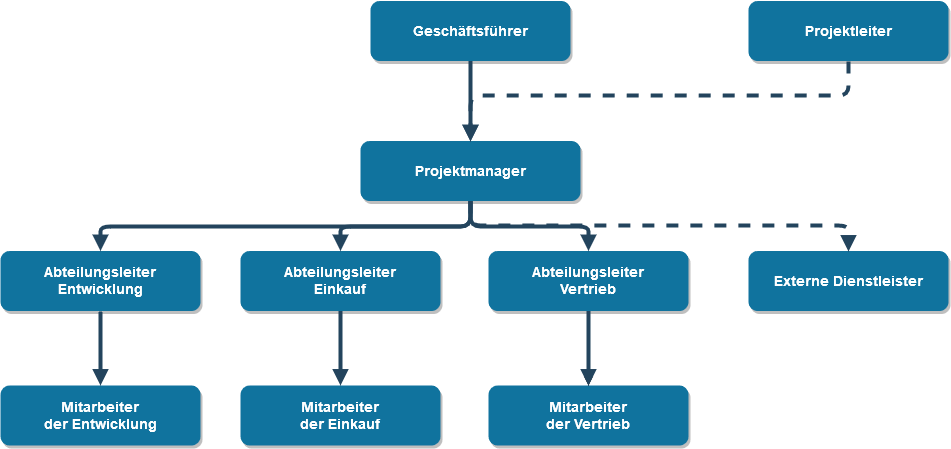
\includegraphics[width=0.8\textwidth]{OBS.png}
    \end{center}
    \caption{Organisation-Breakdown-Strukture}
\end{figure}






